\documentclass[11pt,a4paper,twoside]{epig}

\usepackage[english]{babel}
\usepackage[T1]{fontenc}

\usepackage[utf8]{inputenc}
\usepackage{times}
\usepackage{helvet}

\pagestyle{empty}
\newcommand{\smallitem}{\vspace*{-2mm}\item}
\renewcommand{\baselinestretch}{0.95}
\marginparwidth 0pt 
\evensidemargin 2.2cm 
\oddsidemargin 1.8cm 
\topmargin 0cm 
\textwidth 12cm 
\textheight 19cm

\makeatletter
\renewcommand{\fnum@figure}{\textbf{\fontsize{10}{10}\selectfont\sffamily\figurename~\thefigure}}
\renewcommand{\fnum@table}{\textbf{\fontsize{10}{10}\selectfont\sffamily\tablename~\thetable}}
\makeatother


\newcommand{\auteur}[1]{
	\begin{center}
	{#1}
	\end{center}
}

\newcommand{\titre}[1]{
	\begin{center}
	{\large\bfseries \sffamily {#1}}
	\end{center}
}

\newcommand{\affiliation}[1]{
	\noindent
	{\small{#1}}
}

\usepackage{hyperref}
\usepackage{amsmath}  % Maths
\usepackage{amsfonts} % Maths
\usepackage{amssymb}  % Maths
\usepackage{stmaryrd} % Maths (crochets doubles)

\usepackage{url}     % Mise en forme + liens pour URLs
\usepackage{array}   % Tableaux évolués

\usepackage{prettyref}
\newrefformat{def}{Def.~\ref{#1}}
\newrefformat{fig}{Fig.~\ref{#1}}
\newrefformat{pro}{Property~\ref{#1}}
\newrefformat{pps}{Proposition~\ref{#1}}
\newrefformat{lem}{Lemma~\ref{#1}}
\newrefformat{thm}{Theorem~\ref{#1}}
\newrefformat{sec}{Sect.~\ref{#1}}
\newrefformat{ssec}{Subsect.~\ref{#1}}
\newrefformat{suppl}{Appendix~\ref{#1}}
\newrefformat{eq}{Eq.~\eqref{#1}}
\def\pref{\prettyref}

\usepackage{ntheorem}
\theoremheaderfont{\fontsize{10}{10}\sffamily\bfseries}
%\newtheorem*{example}{Example}{\itshape}{}
\newtheorem{example}{Example}{\itshape}{}
\newtheorem{definition}{Definition}{\itshape}{}

\usepackage{tikz}
\newdimen\pgfex
\newdimen\pgfem
\usetikzlibrary{arrows,shapes,shadows,scopes}
\usetikzlibrary{positioning}
\usetikzlibrary{matrix}
\usetikzlibrary{decorations.text}
\usetikzlibrary{decorations.pathmorphing}



%\input{macros/macros}

% Macros générales
\def\Pint{\textsc{PINT}}

% Notations générales pour PH
\newcommand{\PH}{\mathcal{PH}}
\newcommand{\PHs}{\Sigma}
\newcommand{\PHl}{L}
\newcommand{\PHp}{\textcolor{red}{\mathcal{P}}}
\newcommand{\PHproc}{\mathcal{P}}
\newcommand{\PHa}{\PHh}
\newcommand{\PHh}{\mathcal{H}}
\newcommand{\PHn}{\mathcal{N}}

\newcommand{\PHhitter}{\mathsf{hitter}}
\newcommand{\PHtarget}{\mathsf{target}}
\newcommand{\PHbounce}{\mathsf{bounce}}
\newcommand{\PHsort}{\Sigma}

\def\f#1{\mathsf{#1}}
\def\focals{\f{focals}}
\def\play{\cdot}
\def\configs#1{\mathbb C_{#1\rightarrow a}}

\newcommand{\PHfrappeA}{\rightarrow}
\newcommand{\PHfrappeB}{\Rsh}
\newcommand{\PHfrappe}[3]{#1\PHfrappeA#2\PHfrappeB#3}
\newcommand{\PHfrappebond}[2]{#1\PHfrappeB#2}
\newcommand{\PHobjectif}[2]{\mbox{$#1\PHfrappeB^*\!#2$}}
\newcommand{\PHconcat}{::}
\newcommand{\PHneutralise}{\rtimes}

\def\PHget#1#2{{#1[#2]}}
\newcommand{\PHchange}[2]{(#1 \Lleftarrow #2)}
\newcommand{\PHarcn}[2]{\mbox{$#1\PHneutralise#2$}}
\newcommand{\PHjoue}{\cdot}

\newcommand{\PHetat}[1]{\mbox{$\langle #1 \rangle$}}

% Notations spécifiques à ce papier
\newcommand{\PHdirectpredec}[1]{\PHs^{-1}(#1)}
\newcommand{\PHpredec}[1]{\f{pred}(#1)}
\newcommand{\PHpredecgene}[1]{\f{reg}({#1})}
\newcommand{\PHpredeccs}[1]{\PHpredec{#1} \setminus \Gamma}

\newcommand{\PHincl}[2]{#1 :: #2}

\def\ctx{\varsigma}
\def\ctxOverride{\Cap}
\def\PHstate#1{\langle #1 \rangle}

\def\DEF{\stackrel{\Delta}=}
\def\EQDEF{\stackrel{\Delta}\Leftrightarrow}

\def\intervalless{<_{[]}}

%\input{macros/macros-ph}

% Notations pour le modèle de Thomas (depuis thèse)
\newcommand{\GRN}{\mathcal{GRN}}
\newcommand{\IG}{\mathcal{G}}
\newcommand{\GRNreg}[1]{\Gamma^{-1}(#1)}
\newcommand{\GRNres}[2]{\mathsf{Res}_{#1}(#2)}
\newcommand{\GRNallres}[1]{\mathsf{Res}_{#1}}
\newcommand{\GRNget}[2]{\PHget{#1}{#2}}
\newcommand{\GRNetat}[1]{\PHetat{#1}}

\def\levels{\mathsf{levels}}
\def\levelsA#1#2{\levels_+(#1\rightarrow #2)}
\def\levelsI#1#2{\levels_-(#1\rightarrow #2)}

\newcommand{\Kinconnu}{\emptyset}
\newcommand{\RRGva}[3]{#1 \stackrel{#2}{\longrightarrow} #3}
\newcommand{\RRGgi}{\mathcal{G}}
\newcommand{\RRGreg}[1]{\RRGgi_{#1}}

\tikzstyle{grn}=[every node/.style={circle,draw=black,outer sep=2pt,minimum
                size=15pt,text=black}, node distance=1.5cm]
\tikzstyle{act}=[->,draw=black,thick,color=black]
\tikzstyle{inh}=[>=|,-|,draw=black,thick, text=black,label]
\tikzstyle{inf}=[->,draw=colorinf,thick,color=colorinf]
\tikzstyle{elabel}=[fill=none,text=black, above=-2pt,%sloped,
minimum size=10pt, outer sep=0, font=\scriptsize, draw=none]
\tikzstyle{sg}=[every node/.style={outer sep=2pt,minimum
                size=15pt,text=black}, node distance=2cm]

%\input{macros/macros-grn}

\usepackage{ifthen}
\usepackage{tikz}
\usetikzlibrary{arrows,shapes}

\definecolor{lightgray}{rgb}{0.8,0.8,0.8}
\definecolor{lightgrey}{rgb}{0.8,0.8,0.8}

\tikzstyle{boxed ph}=[]
\tikzstyle{sort}=[fill=lightgray,rounded corners]
\tikzstyle{process}=[circle,draw,minimum size=15pt,fill=white,
font=\footnotesize,inner sep=1pt]
\tikzstyle{black process}=[process, fill=black,text=white, font=\bfseries]
\tikzstyle{gray process}=[process, draw=black, fill=lightgray]
\tikzstyle{current process}=[process, draw=black, fill=lightgray]
\tikzstyle{process box}=[white,draw=black,rounded corners]
\tikzstyle{tick label}=[font=\footnotesize]
\tikzstyle{tick}=[black,-]%,densely dotted]
\tikzstyle{hit}=[->,>=angle 45]
\tikzstyle{selfhit}=[min distance=30pt,curve to]
\tikzstyle{bounce}=[densely dotted,->,>=latex]
\tikzstyle{hl}=[font=\bfseries,very thick]
\tikzstyle{hl2}=[hl]
\tikzstyle{nohl}=[font=\normalfont,thin]

\newcommand{\currentScope}{}
\newcommand{\currentSort}{}
\newcommand{\currentSortLabel}{}
\newcommand{\currentAlign}{}
\newcommand{\currentSize}{}

\newcounter{la}
\newcommand{\TSetSortLabel}[2]{
  \expandafter\repcommand\expandafter{\csname TUserSort@#1\endcsname}{#2}
}
\newcommand{\TSort}[4]{
  \renewcommand{\currentScope}{#1}
  \renewcommand{\currentSort}{#2}
  \renewcommand{\currentSize}{#3}
  \renewcommand{\currentAlign}{#4}
  \ifcsname TUserSort@\currentSort\endcsname
    \renewcommand{\currentSortLabel}{\csname TUserSort@\currentSort\endcsname}
  \else
    \renewcommand{\currentSortLabel}{\currentSort}
  \fi
  \begin{scope}[shift={\currentScope}]
  \ifthenelse{\equal{\currentAlign}{l}}{
    \filldraw[process box] (-0.5,-0.5) rectangle (0.5,\currentSize-0.5);
    \node[sort] at (-0.2,\currentSize-0.4) {\currentSortLabel};
   }{\ifthenelse{\equal{\currentAlign}{r}}{
     \filldraw[process box] (-0.5,-0.5) rectangle (0.5,\currentSize-0.5);
     \node[sort] at (0.2,\currentSize-0.4) {\currentSortLabel};
   }{
    \filldraw[process box] (-0.5,-0.5) rectangle (\currentSize-0.5,0.5);
    \ifthenelse{\equal{\currentAlign}{t}}{
      \node[sort,anchor=east] at (-0.3,0.2) {\currentSortLabel};
    }{
      \node[sort] at (-0.6,-0.2) {\currentSortLabel};
    }
   }}
  \setcounter{la}{\currentSize}
  \addtocounter{la}{-1}
  \foreach \i in {0,...,\value{la}} {
    \TProc{\i}
  }
  \end{scope}
}

\newcommand{\TTickProc}[2]{ % pos, label
  \ifthenelse{\equal{\currentAlign}{l}}{
    \draw[tick] (-0.6,#1) -- (-0.4,#1);
    \node[tick label, anchor=east] at (-0.55,#1) {#2};
   }{\ifthenelse{\equal{\currentAlign}{r}}{
    \draw[tick] (0.6,#1) -- (0.4,#1);
    \node[tick label, anchor=west] at (0.55,#1) {#2};
   }{
    \ifthenelse{\equal{\currentAlign}{t}}{
      \draw[tick] (#1,0.6) -- (#1,0.4);
      \node[tick label, anchor=south] at (#1,0.55) {#2};
    }{
      \draw[tick] (#1,-0.6) -- (#1,-0.4);
      \node[tick label, anchor=north] at (#1,-0.55) {#2};
    }
   }}
}
\newcommand{\TSetTick}[3]{
  \expandafter\repcommand\expandafter{\csname TUserTick@#1_#2\endcsname}{#3}
}

\newcommand{\myProc}[3]{
  \ifcsname TUserTick@\currentSort_#1\endcsname
    \TTickProc{#1}{\csname TUserTick@\currentSort_#1\endcsname}
  \else
    \TTickProc{#1}{#1}
  \fi
  \ifthenelse{\equal{\currentAlign}{l}\or\equal{\currentAlign}{r}}{
    \node[#2] (\currentSort_#1) at (0,#1) {#3};
  }{
    \node[#2] (\currentSort_#1) at (#1,0) {#3};
  }
}
\newcommand{\TSetProcStyle}[2]{
  \expandafter\repcommand\expandafter{\csname TUserProcStyle@#1\endcsname}{#2}
}
\newcommand{\TProc}[1]{
  \ifcsname TUserProcStyle@\currentSort_#1\endcsname
    \myProc{#1}{\csname TUserProcStyle@\currentSort_#1\endcsname}{}
  \else
    \myProc{#1}{process}{}
  \fi
}

\newcommand{\repcommand}[2]{
  \providecommand{#1}{#2}
  \renewcommand{#1}{#2}
}
\newcommand{\THit}[5]{
  \path[hit] (#1) edge[#2] (#3#4);
  \expandafter\repcommand\expandafter{\csname TBounce@#3@#5\endcsname}{#4}
}
\newcommand{\TBounce}[4]{
  (#1\csname TBounce@#1@#3\endcsname) edge[#2] (#3#4)
}

\newcommand{\TState}[1]{
  \foreach \proc in {#1} {
    \node[current process] (\proc) at (\proc.center) {};
  }
}



% Id est
%\newcommand{\ie}{\textit{i.e.} }
\newcommand{\ie}{i.e.\ }
\newcommand{\resp}{resp.\ }

% Césures
\hyphenation{pa-ra-me-tri-za-tion}
\hyphenation{pa-ra-me-tri-za-tions}

\hyphenpenalty 1000

%\newcommand{\FIG}[4]
%{\begin{figure}[!hbt]
%\begin{center}
%\rotatebox{270}{\includegraphics[width=#1]{#2}}
%\caption{\label{fig:#3}#4\vspace{-5mm}}
%\end{center}
%\end{figure}}



\def\thetitle{Introduction to the Process Hitting and inference of its underlying Biological Regulatory Network}
\def\theauthor{Maxime Folschette}

\title{\thetitle}
\author{\theauthor}



\begin{document}

\titre{\thetitle}
\auteur{\theauthor$^{1}$\\Joint work: Loïc Paulevé, Katsumi Inoue, Morgan Magnin, Olivier Roux}
\affiliation{$^1$
LUNAM Universit\'e, \'Ecole Centrale de Nantes, IRCCyN UMR CNRS 6597\\
(Institut de Recherche en Communications et Cybern\'etique de Nantes)\\
1 rue de la No\"e -- B.P. 92101 -- 44321 Nantes Cedex 3, France.\\
\texttt{Maxime.Folschette@irccyn.ec-nantes.fr}
}

\section*{Abstract}
\vspace{-2mm}
In this paper, the Process Hitting (PH), a recently introduced framework to model concurrent processes, is introduced.
It is notably suitable to model Biological Regulatory Networks (BRNs) with partial knowledge
of cooperations by defining the most permissive dynamics.
On the other hand, the qualitative modeling of BRNs has been widely addressed using Ren\'e Thomas'
formalism, which is also depicted.
A translation from PH to Thomas' representation of BRNs is finally presented.
It first relies on an analysis of all regulations to infer the Interaction Graph, then the possible parametrizations.



%\input{parts/intro}
\section{Introduction}
As regulatory phenomena play a crucial role in biological systems, they need to be studied accurately.
Biological Regulatory Networks (BRNs) consist in sets of either positive or negative mutual effects between the components.
Besides continuous models of physicists, often designed through systems of ordinary
differential equations, a discrete modeling approach was initiated by René Thomas in 1973
\cite{Thomas73} allowing the representation of the different levels of a component, such as concentration or expression levels, as integer values.
Nevertheless, these dynamics can be precisely established only with regard to some kind of ``focal points'', related to as Thomas' parameters, indicating the evolutionary tendency of each component.
This modeling has motivated numerous works (e.g., \cite{RiCo07,Naldi09,Siebert06,Ahmad08}),
and other approaches related to our work, which rely on temporal logic~\cite{Khalis09} and constraint programming~\cite{20646302,DBLP:conf/ipcat/CorblinFTCT12},
aim at determining models consistent with partial data on the regulatory structure and dynamics.
While the formal checking of dynamical properties is often limited to small networks because of the
state graph explosion, the main drawback of this framework is the difficulty to specify Thomas'
parameters, especially for large networks.

In order to address the formal checking of dynamical properties within very large BRNs, we recently
introduced in \cite{PMR10-TCSB} a new formalism, named the \emph{``Process Hitting''} (PH), to model
concurrent systems having components with a few qualitative levels.
A PH describes, in an atomic manner, the possible evolutions of a “process” (representing one
component at one level) triggered by the hit of at most one other “process” in the system.
This particular structure makes the formal analysis of BRNs with hundreds of components tractable \cite{PMR12-MSCS}.
PH is suitable, according to the precision of this information, to model BRNs with different levels of abstraction by capturing the most general dynamics.

In \cite{FPIMR12-CMSB} we show that starting from one PH model,
it is possible to find the underlying interactions, then the underlying Thomas' parameters.
This method relies on an exhaustive search of the interactions between components of the PH model,
and an enumeration of the (possibly large) nesting set of valid parameters,
so that the resulting dynamics are ensured to respect the PH dynamics, \ie no spurious transitions are made possible.

The first benefit of our approach is that it makes possible the construction refining of BRNs with a partial and progressively brought knowledge in PH, while being able to export such models in the Thomas' framework.
Our second contribution is to enhance the knowledge of the formal links between both modelings.
The method can be applied to large BRNs (up to 40 components).

\section{Frameworks}\label{sec:frameworks}
%\input{parts/ph}
\subsection{The Process Hitting framework}
\label{ssec:PH}

A Process Hitting (PH) (\pref{def:PH}) gathers a finite number of concurrent \emph{processes}
grouped into a finite set of \emph{sorts}.
A sort stands for a component of the system while a process, which belongs to a unique sort, stands for one of its expression levels.
A process is noted $a_i$ where $a$ is the sort and $i$ is the process identifier within the sort $a$.
At any time, exactly one process of each sort is present; a \emph{state} of the PH corresponds to such a set of processes.
 
The concurrent interactions between processes are defined by a set of
\emph{actions}.
Actions describe the replacement of a process by another of the same sort
conditioned by the presence of at most one other process in the current state.
An action is denoted by $\PHfrappe{a_i}{b_j}{b_k}$, which is read as
``$a_i$ \emph{hits} $b_j$ to make it bounce to $b_k$'',
where $a_i,b_j,b_k$ are processes of sorts $a$ and $b$,
called respectively \emph{hitter}, \emph{target} and
\emph{bounce} of the action.

\begin{definition}[Process Hitting]\label{def:PH}
A \emph{Process Hitting} is a triple $(\PHs,\PHl,\PHa)$:
\begin{itemize}
\item $\PHs = \{a,b,\dots\}$ is the finite set of \emph{sorts};
\item $\PHl = \prod_{a\in\PHs} \PHl_a$ is the set of states with $\PHl_a = \{a_0,\dots,a_{l_a}\}$
the finite set of \emph{processes} of sort $a\in\Sigma$ and $l_a$ a positive integer, with $a\neq b\Rightarrow \PHl_a \cap \PHl_b = \emptyset$;
\item $\PHa = \{ \PHfrappe{a_i}{b_j}{b_k} \in \PHl_a \times \PHl_b \times \PHl_b \mid (a,b) \in \PHs^2
  \wedge b_j\neq b_k \wedge a=b\Rightarrow a_i=b_j\}$ is the finite set of \emph{actions}.
\end{itemize}
\end{definition}

\noindent
Given a state $s\in \PHl$, the process of sort $a\in\PHs$ present in $s$ is denoted by $\PHget{s}{a}$.
An action $h=\PHfrappe{a_i}{b_j}{b_k} \in \PHa$ is \emph{playable} in $s \in L$ if and only if $\PHget{s}{a}=a_i$ and $\PHget{s}{b} = b_j$.
In such a case, $(s\play h)$ stands for the state resulting from the play of the action $h$ in $s$, with
$\PHget{(s\play h)}{b} = b_k$ and $\forall c \in \PHs, c \neq b, \PHget{(s\play h)}{c} = \PHget{s}{c}$.

\paragraph{Modeling cooperation.}
As described in \cite{PMR10-TCSB}, the cooperation between processes to make another process bounce can be
expressed in PH by building a \emph{cooperative sort}.
\pref{fig:runningPH} shows an example of a cooperative sort $bc$ between sorts $b$ and $c$,
defined with 4 processes (one for each sub-state of the presence of processes $b_1$ and $c_1$).
For the sake of clarity, processes of $bc$ are indexed using the sub-state they represent.
Hence, $bc_{01}$ represents the sub-state $\PHstate{b_0,c_1}$, and so on.
Each process of sort $b$ and $c$ hit $bc$ to make it bounce to the process reflecting the status of the sorts $b$
and $c$ (e.g., $\PHfrappe{b_1}{bc_{00}}{bc_{10}}$ and $\PHfrappe{b_1}{bc_{01}}{bc_{11}}$).
Then, to represent the cooperation between processes $b_1$ and $c_1$,
the process $bc_{11}$ hits $a_1$ to make it bounce to $a_2$ instead of
independent hits from $b_1$ and $c_1$.
The same cooperative sort is used to make $b_0$ and $c_0$ cooperate to hit $a_1$ and make it bounce to $a_0$.

\begin{example}
\pref{fig:runningPH} represents a PH $(\PHs,\PHl,\PHa)$ with especially:
$\PHs = \{a,b,c,bc\}$,
$\PHl_a = \{a_0,a_1,a_2\}$,
$\PHl_b = \{b_0, b_1\}$,
$\PHl_c = \{c_0, c_1\}$ and
$\PHl_{bc} = \{bc_{00}, bc_{01}, bc_{10}, bc_{11}\}$.
This example models a BRN where the component $a$ has three qualitative levels, components $b$ and $c$ are Boolean and $bc$ is a cooperative sort.
In this BRN, $a$ inhibits $b$ at level $2$ while $b$ and $c$ activate $a$ with independent actions (e.g. $\PHfrappe{b_0}{a_2}{a_1}$)
or through the cooperative sort $bc$ (e.g. $\PHfrappe{bc_{11}}{a_1}{a_2}$).
Indeed, the reachability of $a_2$ and $a_0$ is conditioned by a cooperation of $b$ and $c$, as explained above.

\begin{figure}[ht]
\centering
\scalebox{0.9}{
\begin{tikzpicture}
\path[use as bounding box] (-2,-5.2) rectangle (7,0.7);

\TSort{(0,0)}{b}{2}{t}
\TSort{(0,-3.8)}{c}{2}{b}
\TSort{(4.5,-3)}{a}{3}{r}

\TSetTick{bc}{0}{00}
\TSetTick{bc}{1}{01}
\TSetTick{bc}{2}{10}
\TSetTick{bc}{3}{11}
\TSort{(-0.5,-2)}{bc}{4}{b}

\THit{b_1}{bend right}{bc_0}{.north}{bc_2}
\THit{b_1}{bend right}{bc_1}{.north}{bc_3}
\THit{b_0}{}{bc_2}{.north west}{bc_0}
\THit{b_0}{}{bc_3}{.north west}{bc_1}

\THit{c_0}{}{bc_1}{.south}{bc_0}
\THit{c_0}{}{bc_3}{.south}{bc_2}
\THit{c_1}{}{bc_0}{.south}{bc_1}
\THit{c_1}{}{bc_2}{.south}{bc_3}

\path[bounce, bend right=25]
\TBounce{bc_2}{}{bc_0}{.north east}
\TBounce{bc_3}{}{bc_1}{.north east}
;
\path[bounce, bend left=80, distance=30]
\TBounce{bc_0}{}{bc_2}{.north}
\TBounce{bc_1}{}{bc_3}{.north}
;
\path[bounce, bend right]
\TBounce{bc_0}{}{bc_1}{.west}
\TBounce{bc_2}{}{bc_3}{.west}
;
\path[bounce, bend left]
\TBounce{bc_3}{}{bc_2}{.east}
\TBounce{bc_1}{}{bc_0}{.east}
;

\THit{bc_3}{thick}{a_1}{.north west}{a_2}
\THit{bc_0}{thick,bend right=130, in=305, distance=140}{a_1}{.south east}{a_0}
\path[bounce, bend left=40]
\TBounce{a_1}{thick}{a_2}{.south west}
\TBounce{a_1}{thick}{a_0}{.north east}
;

\THit{b_0}{thick,bend left,out=50,in=150}{a_2}{.west}{a_1}
\THit{b_1}{thick,bend left,out=80,in=70,distance=100}{a_0}{.east}{a_1}
\path[bounce]
\TBounce{a_2}{thick,bend right=40}{a_1}{.west}
\TBounce{a_0}{thick,bend right=40}{a_1}{.east}
;

\THit{c_0}{thick,bend left,out=270,in=290, distance=115}{a_2}{.east}{a_1}
\THit{c_1}{thick}{a_0}{.north west}{a_1}
\path[bounce]
\TBounce{a_2}{thick,bend left=40}{a_1}{.north east}
\TBounce{a_0}{thick,bend left=40}{a_1}{.south west}
;

\THit{a_2}{bend left, out=290, in=120}{b_1}{.south}{b_0}
\path[bounce, bend left]
\TBounce{b_1}{}{b_0}{.south}
;

\end{tikzpicture}
}

\caption{\label{fig:runningPH}
A PH example with four sorts: three components ($a$, $b$ and $c$) and a cooperative sort ($bc$).
Actions targeting processes of $a$ are in thick lines.
}
\end{figure}
\end{example}

%\input{parts/grn}
\subsection{Thomas' modeling}
Thomas' formalism, here inspired by \cite{Richard06,BernotSemBRN}, lies on two complementary descriptions of the system.
First, the \emph{Interaction Graph} (IG) models the structure of the system by defining the components' mutual influences.
Its nodes represent components, while its edges labeled with a threshold stand for either positive or negative interactions (\pref{def:ig});
$l_a$ denotes the maximum level of a component $a$.

\begin{definition}[Interaction Graph]
\label{def:ig}
An \emph{Interaction Graph} (IG) is a triple $(\Gamma, E_+, E_-)$ where $\Gamma$ is a finite number of \emph{components},
and $E_+$ (\resp $E_-$) $\subset \{a \xrightarrow{t} b \mid a, b \in \Gamma \wedge t \in [1; l_a]\}$
is the set of positive (\resp negative) \emph{regulations} between two nodes, labeled with a \emph{threshold}.
A regulation from $a$ to $b$ is unique.
\end{definition}

\noindent
For an interaction of the IG to take place, the expression level of its head component has to be higher than its threshold; otherwise, the opposite influence is expressed.
For any component $a \in \Gamma$, $\GRNreg{a} = \{ b\in\Gamma\mid \exists b\xrightarrow t a\in E_+\cup E_- \}$
is the set of its regulators.
A \emph{state} $s$ of an IG $(\Gamma, E_+, E_-)$ is an element in $\prod_{a \in \Gamma} [0;l_a]$
and $\GRNget{s}{a}$ refers to the level of component $a$ in $s$.

The specificity of Thomas' approach lies in the use of discrete \emph{parameters} to represent focal level intervals (\pref{def:param}).

\begin{definition}[Discrete parameter $K_{x,A,B}$ and Parametrization $K$]\label{def:param}
Let $x \in \Gamma$ be a given component and $A$ (\resp $B$) $\subset \GRNreg{x}$ a set of its \emph{activators} (\resp \emph{inhibitors}),
such that $A \cup B = \GRNreg{x}$ and $A \cap B = \emptyset$.
The discrete \emph{parameter} $K_{x,A,B} = [i; j]$ is a non-empty interval so that $0 \leq i \leq j \leq l_x$.
With regard to the dynamics, $x$ will tend towards $K_{x,A,B}$ in the states where its activators (\resp inhibitors) are the regulators in set $A$ (\resp $B$).
The complete map $K = (K_{x,A,B})_{x,A,B}$ of discrete parameters for an IG is called a \emph{parametrization} of this IG.
\end{definition}

At last, dynamics are defined in BRN in a unitary and asynchronous way:
from a given state $s$, a transition to another state $s'$ is possible provided that only one component $a$ will evolve of exactly one level towards $K_{a,A,B}$, where $A$ (\resp $B$) is the set of activators (\resp inhibitors) of $a$ in $s$.

\begin{example}
\pref{fig:runningBRN}(left) represents an Interaction Graph $(\Gamma,E_+,E_-)$ with
$\Gamma = \{a, b, c\}$,
$E_+ = \{b \xrightarrow{1} a, c \xrightarrow{1} a\}$ and
$E_- = \{a \xrightarrow{2} b\}$;
hence $\GRNreg{a} = \{b, c\}$.
\pref{fig:runningBRN}(right) gives a possible parametrization on this IG.
In this BRN, the following transitions are possible:
$\GRNetat{a_0, b_1, c_1} \rightarrow \GRNetat{a_1, b_1, c_1} \rightarrow \GRNetat{a_2, b_1, c_1} \rightarrow
\GRNetat{a_2, b_0, c_1} \rightarrow \GRNetat{a_1, b_0, c_1}$,
where $a_i$ is the component $a$ at level $i$.
\end{example}

\begin{figure}[t]
\begin{minipage}{0.4\linewidth}
\centering
\scalebox{1.2}{
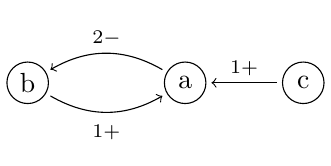
\begin{tikzpicture}[grn]
\path[use as bounding box] (0,-0.7) rectangle (3.5,0.7);
\node[inner sep=0] (a) at (2,0) {a};
\node[inner sep=0] (b) at (0,0) {b};
\node[inner sep=0] (c) at (3.5,0) {c};
\path[->]
  (b) edge[bend right] node[elabel, below=-3pt] {$1+$} (a)
  (c) edge node[elabel, above=-5pt] {$1+$} (a)
  (a) edge[bend right] node[elabel, above=-5pt] {$2-$} (b);
\end{tikzpicture}
}
\end{minipage}
\begin{minipage}{0.6\linewidth}
\centering
\begin{align*}
K_{a,\{b,c\},\emptyset} &= [2 ; 2] & K_{b,\{a\},\emptyset} &= [0 ; 1] \\
K_{a,\{b\},\{c\}} &= [1 ; 1] & K_{b,\emptyset,\{a\}} &= [0 ; 0] \\
K_{a,\{c\},\{b\}} &= [1 ; 1] &&\\
K_{a,\emptyset,\{b,c\}} &= [0 ; 0] & K_{c,\emptyset,\emptyset} &= [0 ; 1]
\end{align*}
\end{minipage}
\caption{\label{fig:runningBRN}
(left)~IG example.
Regulations are represented by the edges labeled with their sign and threshold.
For instance, the edge from $b$ to $a$ is labeled “$1+$”, which stands for: $b \xrightarrow{1} a \in
E_+$.
(right)~Example parametrization of the left IG.
}
\end{figure}



\section{BRN Inference}

In order to infer a complete BRN, one has to find the Interaction Graph (IG) first, as some constraints on the parametrization rely on it.
Inferring the IG is an abstraction step which consists, from atomistic actions of a PH, in determining the global influence of every component on each of its successors.

Given the IG inferred from a PH as presented in the previous section, one can find the discrete parameters that model the behavior of the studied PH using the method presented in the following.
As some parameters may remain undetermined, another step allows to enumerate all parametrizations compatible with the inferred parameters.

%\input{parts/infer-ig}
\subsection{Interaction Graph inference}\label{ssec:infer-IG}
This step assumes that the studied PH defines two types of sorts: the sorts corresponding to BRN components, which will appear in the IG, and the cooperative sorts.
The identification of these two sets of sorts relies on the observation of their possible behavior, which in both cases observe some rules.

Inferring global influences of a predecessor $b$ on a component $a$ requires to find “local influences” from this predecessor first, by considering a given state and changing only the active process of $b$.
The aim is to compare the set of processes towards which the component $a$ will evolve, for each active process of $b$, leaving the active process of all the other sorts unchanged.
Indeed, if after increasing the level of $b$ (\ie activating a higher process of $b$) we notice that $a$ tends to reach a higher (\resp lower) level, we can then deduce that $b$ activates (\resp inhibits) $a$ in this selected state.
Of course, only predecessors of $a$ have to be considered.

This has to be observed on every possible state in order to infer a local influence.
Indeed, if all local influences of $b$ on $a$ are the same (activations or inhibitions) we can deduce that the global influence of $b$ on $a$ is also the same, and the related threshold is the lowest level of $b$ for which we can observe such an influence.
An unsigned edge with no threshold is inferred if two different local influences are found, or in particular cases (when a behavior cannot be represented as a BRN).

\begin{example}
Consider, in the PH of \pref{fig:runningPH}, the sub-state $\PHstate{b_0, c_0, bc_{00}}$ of predecessors of $a$.
In this sub-state, $a$ can be hit by the following actions: $\{\PHfrappe{b_0}{a_2}{a_1}, \PHfrappe{c_0}{a_2}{a_1}, \PHfrappe{bc_{00}}{a_1}{a_0}\}$.
Thus, if $a$ evolves, it will eventually reach process $a_0$.
But if a higher process of $b$ is activated, that is, $b_1$ instead of $b_0$, thus considering the sub-state $\PHstate{b_1, c_0, bc_{10}}$,
then $a$ can be hit by the two following actions: $\{\PHfrappe{b_1}{a_0}{a_1}, \PHfrappe{c_0}{a_2}{a_1}\}$,
and will eventually reach process $a_1$.

Therefore, in this sub-state of predecessors of $a$, $b$ locally activates $a$.
Furthermore, if this analysis is carried for all possible sub-states of predecessors of $a$, only local activations are found,
thus giving: $b \xrightarrow{1} a \in E_+$.
After applying this method to all pairs of influence, the IG given in \pref{fig:runningBRN} is inferred.
\end{example}

%\input{parts/infer-param}
\subsection{Parameters inference}\label{ssec:infer-K}
This subsection presents some results related to the inference of independent discrete parameters from a given PH,
equivalent to those presented in \cite{PMR10-TCSB}.
We suppose in the following that the considered PH is well-formed for parameters inference, \ie its inferred IG does not contain any unsigned edge,
and in each sort, all processes activating (\resp inhibiting) another component share the same behavior.
Let $K_{a,A,B}$ be the parameter we want to infer for a given component $a \in \Gamma$,
and $A \subset \GRNreg{a}$ (\resp $B \subset \GRNreg{a}$) a set of its activators (\resp inhibitors).
This inference, as for the IG inference, relies on the search of focal processes of the component for the given configuration of its regulators.

For each sort $b \in \GRNreg{a}$, we define a context that contains all processes of $b$ activating (\resp inhibiting) $a$ if $b \in A$ (\resp $B$).
From all contexts of all predecessors of $a$, we create a global context that represents the configuration $A,B$ (including the cooperative sorts involved).
The parameter $K_{a,A,B}$ specifies towards which values $a$ eventually evolves as long as this context holds, which is precisely given by the set of focal processes.

\begin{example}
Consider the PH of \pref{fig:runningPH}, from which the IG of \pref{fig:runningBRN} is inferred.
Inferring the parameter $K_{a,\{b,c\},\emptyset}$ requires to understand the behavior of $a$ in the sub-state $\PHstate{b_1, c_1, bc_{11}}$.
In this sub-state, $a$ tends to eventually reach process $a_2$; thus, we can deduce the parameter: $K_{a,\{b,c\},\emptyset} = [2 ; 2]$.
Inferring all parameters leads to the complete parametrization given in \pref{fig:runningBRN}.
\end{example}

\subsection{Admissible parametrizations enumeration}\label{ssec:admissible-K}
The previous inference step may leave several parameters undetermined, due to missing cooperations or behaviors impossible to represent in a BRN.
If it is not possible to change the PH model in order to remove these inconclusive cases,
one can perform a last step to enumerate all valid values for each parameter that could not be inferred given the above results.
We consider that a parameter is valid if any transition it involves in the resulting BRN is allowed by the studied PH by actions that represent this behavior.
We also add some biological constraints on the whole parametrizations, given in \cite{BernotSemBRN}.
These constraints lead to a family of admissible parametrizations which we can enumerate and are ensured to observe a coherent behavior that is included in the original PH.

Answer Set Programming (ASP) \cite{Baral03} turns out to be effective for the enumerative searches developed in this paper,
as it efficiently tackles the inherent complexity of the models we use, thus allowing an efficient execution of the formal tools developed.
Furthermore, ASP finds a particularly interesting application in the research of admissible parametrizations regarding the properties presented above, as this enumeration can be naturally formulated by using of aggregates and constraints.

%\input{parts/example}
\subsection{Implementation}\label{ssec:examples}
The inference method described in this paper has been implemented as a tool named \texttt{ph2thomas}, as part of
\textsc{Pint}\footnote{Available at \url{http://process.hitting.free.fr}}, which gathers PH related
tools.
Our implementation mainly consists of ASP programs that are solved using Clingo\footnote{Available
at \url{http://potassco.sourceforge.net}}.

In the previous sections, we illustrate our results on a toy example considered as a very small network.
But our approach can also successfully handle large PH models of BRNs found in the literature
such as an ERBB receptor-regulated G1/S transition model from \cite{Sahin09} which contains 20
components, and a T-cells receptor model from \cite{Klamt06} which contains 40
components\footnote{Both models are available as examples distributed with \textsc{Pint}.}.
For each model, IG and parameters inferences are performed together in less than a second
on a standard desktop computer.



%\input{parts/discussion}
\section{Conclusion}

This work establishes the abstraction relationship between PH, which is more abstract and allows incomplete knowledge on cooperations, and Thomas' approach for qualitative BRN modeling.
This motivates the concretization of PH models into a set of compatible Thomas' models in order to benefit of the complementary advantages of these two formal frameworks and extract some global information about the influences between components.

As an extension of the present work, we plan to explore new semantics of BRNs to be able to tackle influences currently represented by unsigned edges.

\paragraph{Acknowledgment.}
This work was partially supported by the Fondation Centrale Initiatives.



\begin{thebibliography}{10}

\bibitem{Ahmad08}
Jamil Ahmad, Olivier Roux, Gilles Bernot, Jean-Paul Comet, and Adrien Richard.
\newblock Analysing formal models of genetic regulatory networks with delays.
\newblock {\em International Journal of Bioinformatics Research and
  Applications (IJBRA)}, 4(2), 2008.

\bibitem{Baral03}
Chitta Baral.
\newblock {\em Knowledge Representation, Reasoning and Declarative Problem
  Solving}.
\newblock Cambridge University Press, 2003.

\bibitem{BernotSemBRN}
Gilles Bernot, Franck Cassez, Jean-Paul Comet, Franck Delaplace, C{\'e}line
  M{\"u}ller, and Olivier Roux.
\newblock Semantics of biological regulatory networks.
\newblock {\em Electronic Notes in Theoretical Computer Science}, 180(3):3 --
  14, 2007.

\bibitem{20646302}
Fabien Corblin, Eric Fanchon, and Laurent Trilling.
\newblock Applications of a formal approach to decipher discrete genetic
  networks.
\newblock {\em BMC Bioinformatics}, 11(1):385, 2010.

\bibitem{DBLP:conf/ipcat/CorblinFTCT12}
Fabien Corblin, Eric Fanchon, Laurent Trilling, Claudine Chaouiya, and Denis
  Thieffry.
\newblock Automatic inference of regulatory and dynamical properties from
  incomplete gene interaction and expression data.
\newblock In {\em IPCAT}, volume 7223 of {\em LNCS}, pages 25--30. Springer,
  2012.

\bibitem{FPIMR12-CMSB}
Maxime Folschette, Loïc Paulevé, Katsumi Inoue, Morgan Magnin, and Olivier
  Roux.
\newblock Concretizing the process hitting into biological regulatory networks.
\newblock In David Gilbert and Monika Heiner, editors, {\em Computational
  Methods in Systems Biology}, Lecture Notes in Computer Science, pages
  166--186. Springer Berlin Heidelberg, 2012.

\bibitem{Khalis09}
Z.~Khalis, J.-P. Comet, A.~Richard, and G.~Bernot.
\newblock The {SMBioNet} method for discovering models of gene regulatory
  networks.
\newblock {\em Genes, Genomes and Genomics}, 3(special issue 1):15--22, 2009.

\bibitem{Klamt06}
Steffen Klamt, Julio Saez-Rodriguez, Jonathan Lindquist, Luca Simeoni, and
  Ernst Gilles.
\newblock A methodology for the structural and functional analysis of signaling
  and regulatory networks.
\newblock {\em BMC Bioinformatics}, 7(1):56, 2006.

\bibitem{Naldi09}
Aurélien Naldi, Elisabeth Remy, Denis Thieffry, and Claudine Chaouiya.
\newblock A reduction of logical regulatory graphs preserving essential
  dynamical properties.
\newblock In {\em Computational Methods in Systems Biology}, volume 5688 of
  {\em LNCS}, pages 266--280. Springer, 2009.

\bibitem{PMR10-TCSB}
{L}o{\"i}c {P}aulev{\'e}, {M}organ {M}agnin, and {O}livier {R}oux.
\newblock Refining dynamics of gene regulatory networks in a stochastic
  $\pi$-calculus framework.
\newblock In {\em Transactions on Computational Systems Biology XIII}, pages
  171--191. Springer, 2011.

\bibitem{PMR12-MSCS}
{L}o{\"i}c. Paulev\'{e}, Morgan Magnin, and Olivier Roux.
\newblock Static analysis of biological regulatory networks dynamics using
  abstract interpretation.
\newblock {\em Mathematical Structures in Computer Science}, in press, 2012.
\newblock Preprint: \url{http://loicpauleve.name/mscs.pdf}.

\bibitem{RiCo07}
Adrien Richard and Jean-Paul Comet.
\newblock Necessary conditions for multistationarity in discrete dynamical
  systems.
\newblock {\em Discrete Applied Mathematics}, 155(18):2403 -- 2413, 2007.

\bibitem{Richard06}
Adrien Richard, Jean-Paul Comet, and Gilles Bernot.
\newblock {\em Modern Formal Methods and App.}, chapter Formal Methods for
  Modeling Biological Regulatory Networks, pages 83--122.
\newblock 2006.

\bibitem{Sahin09}
Ozgur Sahin, Holger Frohlich, Christian Lobke, Ulrike Korf, Sara Burmester,
  Meher Majety, Jens Mattern, Ingo Schupp, Claudine Chaouiya, Denis Thieffry,
  Annemarie Poustka, Stefan Wiemann, Tim Beissbarth, and Dorit Arlt.
\newblock Modeling {ERBB} receptor-regulated {G}1/{S} transition to find novel
  targets for de novo trastuzumab resistance.
\newblock {\em BMC Systems Biology}, 3(1), 2009.

\bibitem{Siebert06}
Heike Siebert and Alexander Bockmayr.
\newblock Incorporating time delays into the logical analysis of gene
  regulatory networks.
\newblock In {\em Computational Methods in Systems Biology}, volume 4210 of
  {\em LNCS}, pages 169--183. Springer, 2006.

\bibitem{Thomas73}
Ren{\'e} Thomas.
\newblock Boolean formalization of genetic control circuits.
\newblock {\em Journal of Theoretical Biology}, 42(3):563 -- 585, 1973.

\end{thebibliography}



\end{document}
